\begin{frame}{}
	\maketitle
\end{frame}
\note[itemize]{
	\item
}

\begin{frame}{La reina de la Costa Negra}
	\begin{columns}
		\column[t]{0.5\textwidth}
		\begin{figure}[htb]
			\centering
			\includegraphics[width=0.8\textwidth]{img/Intro}
			\caption{Mark Schultz}
		\end{figure}
		\column[t]{0.5\textwidth}
		\begin{itemize}
			\item Una historia corta de Robert E. Howard
			\item Una de sus mejores historias
			\item Espada y hechicería
		\end{itemize}
	\end{columns}
\end{frame}
\note[itemize]{
	\item
}

\begin{frame}{Publicación}
	\begin{columns}
		\column[t]{0.4\textwidth}
		\begin{figure}[htb]
			\centering
			\includegraphics[width=0.5\textwidth]{img/Weird_Tales_1934-05}
			\caption{Mayo de 1934}
		\end{figure}
		\column[t]{0.6\textwidth}
		\begin{itemize}
			\item Publicada por primera vez en Weird Tales
			\item La \say{historia de portada} por Margaret Brundage
			\item Alrededor de unas 20 páginas
			\begin{itemize}
				\item 11300 palabras en Ingles
				\item 13200 palabras en Español
				\item Lectura en 70-100 minutos
			\end{itemize}
			\item Una historia de su personaje mas famoso: Conan el bárbaro
			\item Muchas veces publicada en Español y en el idioma original
		\end{itemize}
	\end{columns}
\end{frame}
\note[itemize]{
	\item Mencioanr que esta fué la historia de portada
}

\begin{frame}{La primera ilustración}
	\begin{columns}
		\column[t]{0.4\textwidth}
		\begin{figure}[htb]
			\centering
			\includegraphics[width=0.75\textwidth]{img/HughRankinReinaCostaNegra}
			\caption{Hugh Rankin}
		\end{figure}
		\column[t]{0.6\textwidth}
		\begin{itemize}
			\item Esta ilustración acompaña a la primera edición de la historia

		\end{itemize}
	\end{columns}
\end{frame}
\note[itemize]{
	\item Mencionar que entonce entre esta y la historia de portada se reparten el derecho a ser la primera ilustración
}

\begin{frame}{Orden de publicación del ciclo de Conan}
	\begin{figure}[htb]
		\centering
		\includegraphics[width=0.32\textwidth]{img/OrdenPublicacion}
	\end{figure}
\end{frame}
\note[itemize]{
	\item La reina de la costa Negra forma parte del ciclo de Conan, que consta de 18 a 25 historias de REH, dependiendo de cómo queramos contarlas.
	\item Si solo se cuentan historias publicadas en la vida de REH, son 18 (o 17 dependiendo de si se cuenta o no \say{La hija del gigante helado}).
	\item Si se añaden la historias que fueron rechazadas por los editores durante la vida de REH, y luego publicadas después de su muerte; así como fragmentos que el autor dejó inconclusos y que fueron --muchos años después-- terminados y publicados por otros autores, ahí la cuenta sube a 25.
}

\begin{frame}{Cronología ficticia del personaje}
	\begin{figure}[htb]
		\centering
		\includegraphics[width=0.85\textwidth]{img/Cronologias}
	\end{figure}
\end{frame}
\note[itemize]{
	\item Esta es una historia de la edad temprana de Conan.
	\item Es segun Joe Marek el segundo estereotipo que representa Conan.
	\item Pasa de ser un aventurero solitario a ser un lider y tener un proposito
}

\begin{frame}{Espacio en la edad Hiboria}
	\begin{figure}[htp]
		\centering
		\begin{subfigure}[b]{0.2\textwidth}
			\includegraphics[width=\textwidth]{img/mapas/inset}
			%\caption{Silvio \say{Sal} Buscema}
		\end{subfigure}
		~
		\begin{subfigure}[b]{0.5\textwidth}
			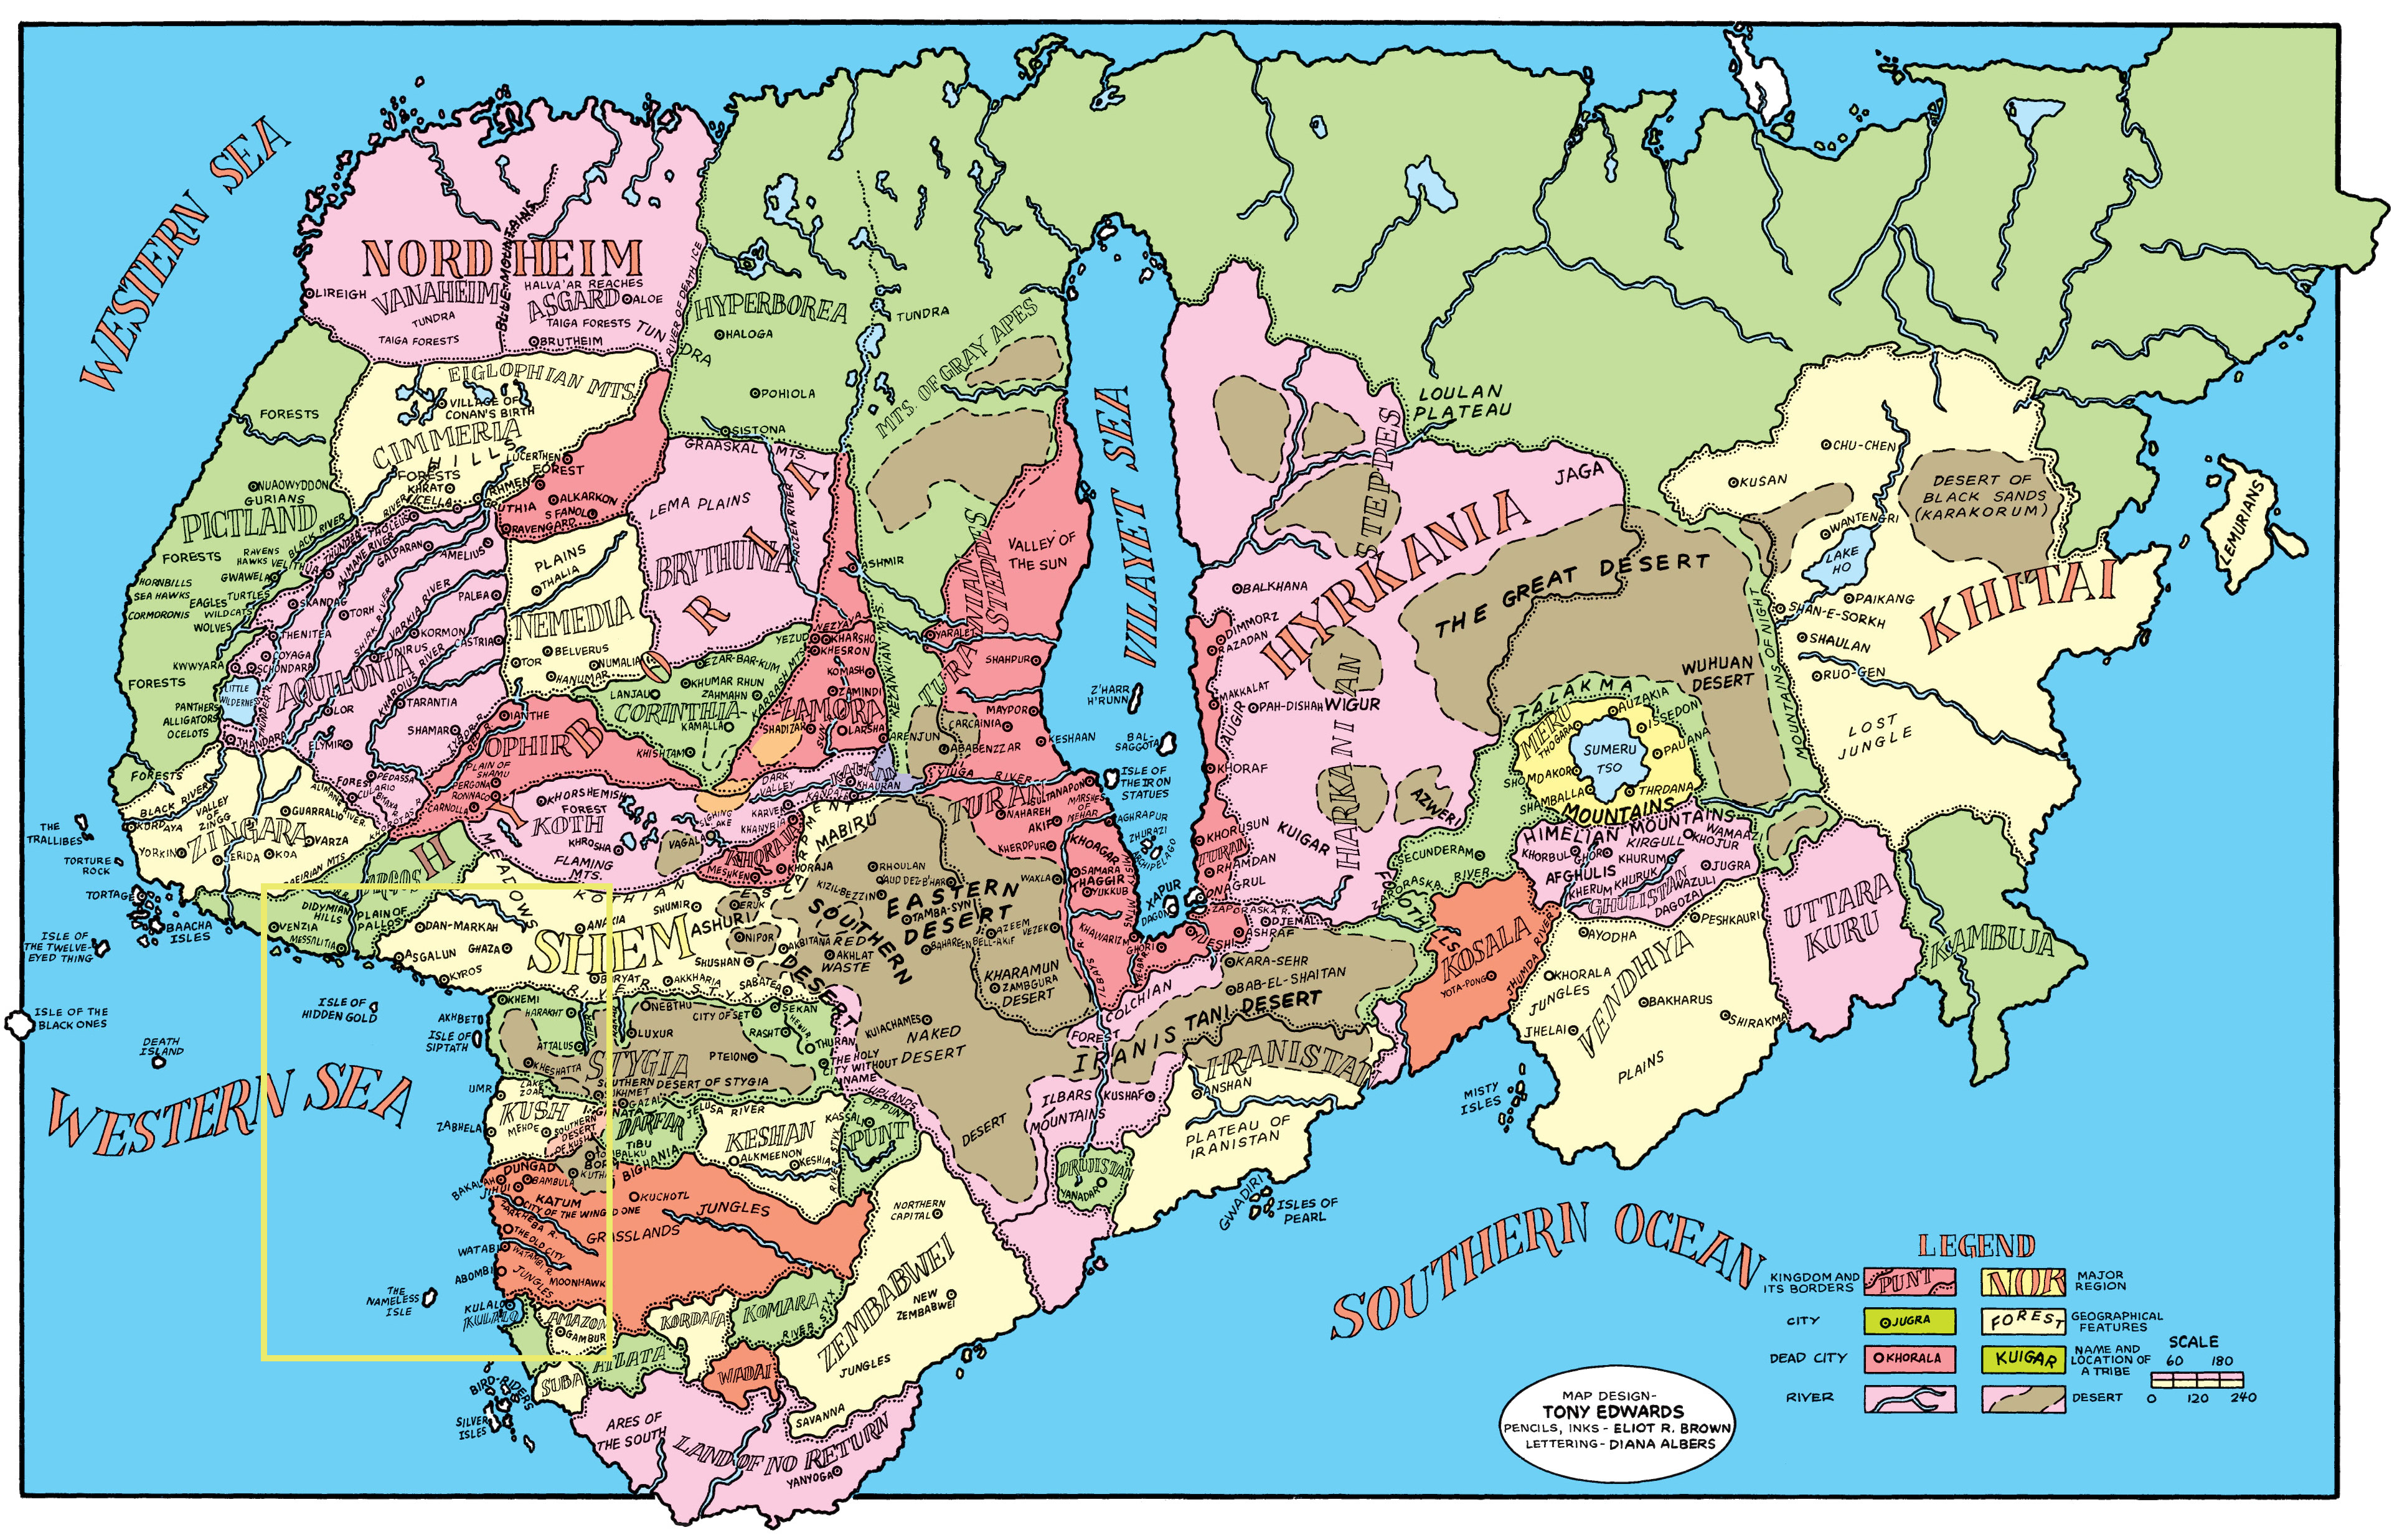
\includegraphics[width=\textwidth]{img/mapas/todo}
			%\caption{Barry Windsor Smith}
		\end{subfigure}
		\caption{La costa Negra}
	\end{figure}
\end{frame}
\note[itemize]{
	\item Recordemos que estamos hablando de Goegrafía imaginaria, y no canonica
	\item La aventura pasa por un espacio geografico muy amplio
	\item Empieza en un puerto de Shem y Conan pasa años recorriendo la llamada \say{Costa Negra}
	\item El barco se llama Argos, como si quisieramos decir que venia originalmente de Argos
	\item La aventura termina en el Rio Zagreba
}

\section{Adaptaciones}
\note[itemize]{
	\item
}

\begin{frame}{Conan the barbarian}
	\begin{columns}
		\column[t]{0.5\textwidth}
		\begin{figure}[htb]
			\centering
			\begin{subfigure}[b]{0.4\textwidth}
				\includegraphics[width=\textwidth]{img/CTB058}
				\caption{58}
			\end{subfigure}
			~
			\begin{subfigure}[b]{0.4\textwidth}
				\includegraphics[width=\textwidth]{img/CTB100}
				\caption{100}
			\end{subfigure}
		\end{figure}
		\column[t]{0.5\textwidth}
		\begin{itemize}
			\item 58: 31 de Diciembre de 1975
			\begin{description}
				\item[Dibujante:] Jhon Buscema
				\item[Entintador:] Steve Gan
				\item[Escritor:] Roy Thomas
				\item[Letrista:] Costanza E. Rosen
				\item[Colorista:] Michele Wolfman
			\end{description}
		\end{itemize}
		\begin{itemize}
			\item 100: 30 de Junio de 1979
			\begin{description}
				\item[Dibujantes:] Jhon Buscema y Ernie Chan
				\item[Entintador:] Steve Gan
				\item[Escritor:] Roy Thomas
				\item[Letrista:] Joe Rosen
				\item[Colorista:] George Roussos
			\end{description}
		\end{itemize}
	\end{columns}
\end{frame}
\note[itemize]{
	\item
}


\begin{frame}{Conan The Barbarian}
	\begin{columns}
		\column[t]{0.5\textwidth}
		\begin{figure}[htp]
			\centering
			\begin{subfigure}[b]{0.23\textwidth}
				\includegraphics[width=\textwidth]{img/DH-CTB-01}
			\end{subfigure}
			~
			\begin{subfigure}[b]{0.23\textwidth}
				\includegraphics[width=\textwidth]{img/DH-CTB-02}
			\end{subfigure}
			~
			\begin{subfigure}[b]{0.23\textwidth}
				\includegraphics[width=\textwidth]{img/DH-CTB-03}
			\end{subfigure}
			\\
			\begin{subfigure}[b]{0.23\textwidth}
				\includegraphics[width=\textwidth]{img/DH-CTB-22}
			\end{subfigure}
			~
			\begin{subfigure}[b]{0.23\textwidth}
				\includegraphics[width=\textwidth]{img/DH-CTB-23}
			\end{subfigure}
			~
			\begin{subfigure}[b]{0.23\textwidth}
				\includegraphics[width=\textwidth]{img/DH-CTB-24}
			\end{subfigure}
		\end{figure}
		\column[t]{0.5\textwidth}
		\begin{itemize}
			\item Publicado por de Dark Horse
			\item Números 1-3 y 22-24
			\item Feb-Abr 2012 y Nov-Ene 2014
			\item Créditos:
			\begin{description}
				\item[Artista:] Becky Cloonan (1-3)
				\item[Artista:] Riccardo Burchielli (22-24)
				\item[Escritor:] Brian Wood
				\item[Colorista:] Dave Steward
				\item[Portada:] Massimo Carnevale
				\item[Letrista:] Richard Starkings
			\end{description}
		\end{itemize}
	\end{columns}
\end{frame}
\note[itemize]{
	\item
}

\begin{frame}{The cimmerian}
	\begin{columns}
		\column[t]{0.5\textwidth}
		\begin{figure}[htb]
			\centering
			\begin{subfigure}[b]{0.4\textwidth}
				\includegraphics[width=\textwidth]{img/ablazeTC1}
			\end{subfigure}
			~
			\begin{subfigure}[b]{0.4\textwidth}
				\includegraphics[width=\textwidth]{img/ablazeTC2}
			\end{subfigure}
			\caption{Octubre y Noviembre 2019}
		\end{figure}
		\column[t]{0.5\textwidth}
		\begin{itemize}
			\item Publicado por Ablaze
			\item Dos números seguidos
			\item Créditos:
			\begin{description}
				\item[Dibujante:] Pierre Alary
				\item[Portada:] Jason Metcalf (1)
				\item[Portada:]  Sunghan Yune (2)
				\item[Escritor:] Jean-David Morvan
				\item[Letrista:] Dezi Sienty
				\item[Colorista:] Sergio Sedyas
			\end{description}
		\end{itemize}
	\end{columns}
\end{frame}
\note[itemize]{
	\item
}


\section{Resumen}
\note[itemize]{
	\item
}

\begin{frame}{}
	\begin{columns}
		\column[t]{0.5\textwidth}
		\begin{figure}[htb]
			\centering
			\includegraphics[width=0.9\textwidth]{img/res/01}
			\caption{El Maul}
		\end{figure}
		\column[t]{0.5\textwidth}
		\begin{figure}[htb]
			\centering
			\includegraphics[width=0.9\textwidth]{img/res/02}
			\caption{Una taberna}
		\end{figure}
	\end{columns}
\end{frame}
\note{

}


\section{Personajes}
\note[itemize]{
	\item
}

\begin{frame}{Conan}
	\begin{columns}
		\column[t]{0.4\textwidth}
		\begin{itemize}
			\item Un bárbaro del norte
			\item Hombre de acción: guerrero por excelencia
			\item Inocente para su entorno: La civilización le parece extraña y sin sentido
			\item Con los ideales de su pueblo arraigados
			\item Tiene tendencia a la reflexión e introspección
			\item Pero acepta la vida con una filosofía clara y practica
		\end{itemize}
		\column[t]{0.6\textwidth}
		\begin{figure}[htp]
			\centering
			\begin{subfigure}[b]{0.3\textwidth}
				\includegraphics[width=\textwidth]{img/conan/CTB}
			\end{subfigure}
			~
			\begin{subfigure}[b]{0.27\textwidth}
				\includegraphics[width=\textwidth]{img/conan/DH}
			\end{subfigure}
			~
			\begin{subfigure}[b]{0.23\textwidth}
				\includegraphics[width=\textwidth]{img/conan/TSSC}
			\end{subfigure}
		\end{figure}
	\end{columns}
\end{frame}
\note[itemize]{
	\item
}

\begin{frame}{Belit}
	\begin{columns}
		\column[t]{0.4\textwidth}
		\begin{itemize}
			\item Líder de los piratas, que la veneran como diosa y nunca cuestionan sus ordenes
			\item De mentalidad práctica
			\item La autodenominada \say{Reina de la costa negra}
			\item De sentimientos profundos y salvajes
			\item Estratega y guerrera
		\end{itemize}
		\column[t]{0.6\textwidth}
		\begin{figure}[htp]
			\centering
			\begin{subfigure}[b]{0.3\textwidth}
				\includegraphics[width=\textwidth]{img/conan/CTB}
			\end{subfigure}
			~
			\begin{subfigure}[b]{0.27\textwidth}
				\includegraphics[width=\textwidth]{img/conan/DH}
			\end{subfigure}
			~
			\begin{subfigure}[b]{0.23\textwidth}
				\includegraphics[width=\textwidth]{img/conan/TSSC}
			\end{subfigure}
		\end{figure}
	\end{columns}
\end{frame}
\note[itemize]{
	\item
}

\begin{frame}{Tito}
	\begin{columns}
		\column[t]{0.4\textwidth}
		\begin{itemize}
			\item Capitán del Argos
			\item Conocedor de su oficio, de la civilización y su entorno
			\item Un comerciante pacífico
			\item Un hombre práctico
		\end{itemize}
		\column[t]{0.6\textwidth}
		\begin{figure}[htp]
			\centering
			\begin{subfigure}[b]{0.3\textwidth}
				\includegraphics[width=\textwidth]{img/conan/CTB}
			\end{subfigure}
			~
			\begin{subfigure}[b]{0.27\textwidth}
				\includegraphics[width=\textwidth]{img/conan/DH}
			\end{subfigure}
			~
			\begin{subfigure}[b]{0.23\textwidth}
				\includegraphics[width=\textwidth]{img/conan/TSSC}
			\end{subfigure}
		\end{figure}
	\end{columns}
\end{frame}
\note[itemize]{
	\item
}


\begin{frame}{El guardián de las ruinas}
	\begin{columns}
		\column[t]{0.4\textwidth}
		\begin{itemize}
			\item Miembro de una raza primordial y antigua que se ha sumido en la decadencia por siglos
			\item Poseedor de fuerza sobrehumana y salvaje
			\begin{itemize}
			   \item pero malvado y astuto
			   \item con conocimientos de magia
		    \end{itemize}
		\end{itemize}
		\column[t]{0.6\textwidth}
		\begin{figure}[htp]
			\centering
			\begin{subfigure}[b]{0.3\textwidth}
				\includegraphics[width=\textwidth]{img/conan/CTB}
			\end{subfigure}
			~
			\begin{subfigure}[b]{0.27\textwidth}
				\includegraphics[width=\textwidth]{img/conan/DH}
			\end{subfigure}
			~
			\begin{subfigure}[b]{0.23\textwidth}
				\includegraphics[width=\textwidth]{img/conan/TSSC}
			\end{subfigure}
		\end{figure}
	\end{columns}
\end{frame}
\note[itemize]{
	\item
}

\begin{frame}{El rio Zarkheba}
	\begin{columns}
		\column[t]{0.4\textwidth}
		\begin{itemize}
			\item Su nombre significa muerte
			\item Rio maldito:
			\begin{itemize}
				\item de aguas putrefactas y venenosas
				\item Habitado por serpientes gigantes que devoran hombres
			\end{itemize}
			\item Probablemente la causa del declive de la civilización primigenia
		\end{itemize}
		\column[t]{0.6\textwidth}
		\begin{figure}[htp]
			\centering
			\begin{subfigure}[b]{0.3\textwidth}
				\includegraphics[width=\textwidth]{img/conan/CTB}
			\end{subfigure}
			~
			\begin{subfigure}[b]{0.27\textwidth}
				\includegraphics[width=\textwidth]{img/conan/DH}
			\end{subfigure}
			~
			\begin{subfigure}[b]{0.23\textwidth}
				\includegraphics[width=\textwidth]{img/conan/TSSC}
			\end{subfigure}
		\end{figure}
	\end{columns}
\end{frame}
\note[itemize]{
	\item
}

\begin{frame}{El loto negro}
	\begin{columns}
		\column[t]{0.4\textwidth}
		\begin{itemize}
			\item Planta cuyo aroma induce:
			\begin{itemize}
				\item la parálisis y el sueño
				\item alucinaciones y pesadillas
			\end{itemize}
			\item Parecen moverse sin que sople el viento
		\end{itemize}
		\column[t]{0.6\textwidth}
		\begin{figure}[htp]
			\centering
			\begin{subfigure}[b]{0.3\textwidth}
				\includegraphics[width=\textwidth]{img/conan/CTB}
			\end{subfigure}
			~
			\begin{subfigure}[b]{0.27\textwidth}
				\includegraphics[width=\textwidth]{img/conan/DH}
			\end{subfigure}
			~
			\begin{subfigure}[b]{0.23\textwidth}
				\includegraphics[width=\textwidth]{img/conan/TSSC}
			\end{subfigure}
		\end{figure}
	\end{columns}
\end{frame}
\note[itemize]{
	\item
}

\begin{frame}{Las hienas}
	\begin{columns}
		\column[t]{0.4\textwidth}
		\begin{itemize}
			\item Sirvientes del guardián de las ruinas
			\item Con tamaño y fuerza sobrenatural
			\item Antes fueron hombres
			\begin{itemize}
				\item transformados en bestias por la hechicería
			\end{itemize}
		\end{itemize}
		\column[t]{0.6\textwidth}
		\begin{figure}[htp]
			\centering
			\begin{subfigure}[b]{0.3\textwidth}
				\includegraphics[width=\textwidth]{img/conan/CTB}
			\end{subfigure}
			~
			\begin{subfigure}[b]{0.27\textwidth}
				\includegraphics[width=\textwidth]{img/conan/DH}
			\end{subfigure}
			~
			\begin{subfigure}[b]{0.23\textwidth}
				\includegraphics[width=\textwidth]{img/conan/TSSC}
			\end{subfigure}
		\end{figure}
	\end{columns}
\end{frame}
\note[itemize]{
	\item
}

\begin{frame}{M’Gora}
	\begin{columns}
		\column[t]{0.4\textwidth}
		\begin{itemize}
			\item Miembro de la tripulación de \say{La Tigresa}
			\item Segundo al comando (tercero cuando se une Conan)
			\item Guerrero fiel y amigo de Conan
			\begin{itemize}
				\item que pierde la razón y muere\ldots
				\item a manos de Conan
			\end{itemize}
		\end{itemize}
		\column[t]{0.6\textwidth}
		\begin{figure}[htp]
			\centering
			\begin{subfigure}[b]{0.3\textwidth}
				\includegraphics[width=\textwidth]{img/conan/CTB}
			\end{subfigure}
			~
			\begin{subfigure}[b]{0.27\textwidth}
				\includegraphics[width=\textwidth]{img/conan/DH}
			\end{subfigure}
			~
			\begin{subfigure}[b]{0.23\textwidth}
				\includegraphics[width=\textwidth]{img/conan/TSSC}
			\end{subfigure}
		\end{figure}
	\end{columns}
\end{frame}
\note[itemize]{
	\item
}

\begin{frame}{N'Yaga}
	\begin{columns}
		\column[t]{0.4\textwidth}
		\begin{itemize}
			\item Miembro de la tripulación de \say{La Tigresa}
			\item Chaman y curandero
			\item Consejero de Belit
			\item Es el primero que advierte el peligro mortal
		\end{itemize}
		\column[t]{0.6\textwidth}
		\begin{figure}[htp]
			\centering
			\begin{subfigure}[b]{0.3\textwidth}
				\includegraphics[width=\textwidth]{img/conan/CTB}
			\end{subfigure}
			~
			\begin{subfigure}[b]{0.27\textwidth}
				\includegraphics[width=\textwidth]{img/conan/DH}
			\end{subfigure}
			~
			\begin{subfigure}[b]{0.23\textwidth}
				\includegraphics[width=\textwidth]{img/conan/TSSC}
			\end{subfigure}
		\end{figure}
	\end{columns}
\end{frame}
\note[itemize]{
	\item
}

\begin{frame}{La Tigresa}
	\begin{columns}
		\column[t]{0.4\textwidth}
		\begin{itemize}
			\item El barco pirata que comanda Belit
			\item Parece estar ligado al destino de su capitana
			\item Representa el mar, la libertad de la vida de saqueo
			\item Esta atado a Belit, cuando ella muere se vuelve su tumba
		\end{itemize}
		\column[t]{0.6\textwidth}
		\begin{figure}[htp]
			\centering
			\begin{subfigure}[b]{0.3\textwidth}
				\includegraphics[width=\textwidth]{img/conan/CTB}
			\end{subfigure}
			~
			\begin{subfigure}[b]{0.27\textwidth}
				\includegraphics[width=\textwidth]{img/conan/DH}
			\end{subfigure}
			~
			\begin{subfigure}[b]{0.23\textwidth}
				\includegraphics[width=\textwidth]{img/conan/TSSC}
			\end{subfigure}
		\end{figure}
	\end{columns}
\end{frame}
\note[itemize]{
	\item
}

\section{Citas interesantes}
\note[itemize]{
	\item
}

\begin{frame}{Las leyes de los hombres civilizados}
	\begin{exampleblock}{}
		… the judge squalled that I had shown contempt for the court, and that I should be hurled into a dungeon to rot until I betrayed my friend. So then, seeing they were all mad, I drew my sword and cleft the judge’s skull;
	\end{exampleblock}

	\begin{itemize}
		\item \textit{ \say{El juez dijo gritando que yo había manifestado un profundo desprecio hacia el tribunal y que debía ser encerrado en una mazmorra para que me pudriera allí, hasta que traicionara a mi amigo. Por consiguiente, y viendo que estaban todos locos, desenvainé mi espada y le partí la cabeza al juez;} }
	\end{itemize}
\end{frame}
\note[itemize]{
	\item
}

\begin{frame}{Promesa mas allá de la muerte}
	\begin{exampleblock}{}
		my love is stronger than any death! I have lain in your arms, panting with the violence of our love; you have held and crushed and conquered me, drawing my soul to your lips with the fierceness of your bruising kisses. My heart is welded to your heart, my soul is part of your soul! Were I still in death and you fighting for life, I would come back from the abyss to aid you–aye, whether my spirit floated with the purple sails on the crystal sea of paradise, or writhed in the molten flames of hell! I am yours, and all the gods and all their eternities shall not sever us!
	\end{exampleblock}

	\begin{itemize}
		\item \textit{ \say{¡Sé que mi amor es más fuerte que la muerte! Me has estrechado en tus brazos, jadeando con la violencia de nuestro amor; me has cogido y estrujado y me has conquistado, atrayéndome el alma a tus labios con la violencia de tus hirientes besos. ¡Mi corazón está soldado al tuyo; mi alma es parte de tu alma! ¡Si yo muero y tú tuvieras que luchar por tu vida, yo volvería del abismo para ayudarte; sí, lo haría tanto si mi espíritu flotara bajo las velas purpúreas del mar cristalino del paraíso, como si se retorciese entre las llamas del infierno! ¡Soy tuya, y ni los dioses ni la eternidad podrán separarnos!} }
	\end{itemize}
\end{frame}
\note[itemize]{
	\item
}

\begin{frame}{La vida es una ilusión}
	\begin{exampleblock}{}
		 I know this: if life is illusion, then I am no less an illusion, and being thus, the illusion is real to me. I live, I burn with life, I love, I slay, and am content.
	\end{exampleblock}

	\begin{itemize}
		\item \textit{ \say{Yo sólo sé esto: que si la vida es ilusión, yo no soy más que eso, una ilusión, y ella, por consiguiente, es una realidad para mí. Estoy vivo, me consume la pasión, amo y mato; con eso me doy por contento.} }
	\end{itemize}
\end{frame}
\note[itemize]{
	\item
}

\begin{frame}{Los dioses del norte}
	\begin{exampleblock}{}
		Their chief is Crom. He dwells on a great mountain. What use to call on him? Little he cares if men live or die. Better to be silent than to call his attention to you; he will send you dooms, not fortune! He is grim and loveless, but at birth he breathes power to strive and slay into a man’s soul. What else shall men ask of the gods?
	\end{exampleblock}

	\begin{itemize}
		\item \textit{ \say{El dios principal es Crom, que vive en una gran montaña. Pero de nada vale invocarlo. Le importa muy poco si los hombres viven o mueren. ¡Es mejor callar que reclamar su atención, ya que suele enviar desdichas y no fortuna! Es implacable y sin compasión, pero infunde poder para luchar y matar en el momento de nacer. ¿Qué más puede pedir un ser humano?} }
	\end{itemize}
\end{frame}
\note[itemize]{
	\item
}

\begin{frame}{La canción de Belit}
	\begin{exampleblock}{}
		Believe green buds awaken in the spring.

		That autumn paints the leaves with somber fire;

		Believe I held my heart inviolate

		To lavish on one man my hot desire.
	\end{exampleblock}

	\begin{itemize}
		\item \textit{ \say{Creedme, los verdes brotes despiertan en primavera \\
				y el otoño pinta las hojas con un fuego sombrío; \\
				creedme, yo aún conservo virgen mi corazón \\
				para prodigar mis ardientes deseos a un solo hombre.} }
	\end{itemize}
\end{frame}
\note[itemize]{
	\item
}

\section{Tropes literarios}
\note[itemize]{
	\item
}

\begin{frame}{Espada y hechizeria}
	\begin{columns}
		\column[t]{0.4\textwidth}
		\begin{itemize}
			\item Aventura que no genero un cambio
			\item La espada: la justicia; la hechicería: el mal
			\item Mito de Circe: hechicero convirtió a guerreros en animales/esclavos
		\end{itemize}
		\column[t]{0.6\textwidth}
		\begin{figure}[htb]
			\centering
			\includegraphics[width=0.8\textwidth]{img/tributos/elephant07}
			\caption{Abe Papakhian}
		\end{figure}
	\end{columns}
\end{frame}
\note[itemize]{
	\item
}

\begin{frame}{Sueños reveladores}
	\begin{columns}
		\column[t]{0.4\textwidth}
		\begin{itemize}
			\item Una parte importante de la trama es revelada en un sueño
			\item El sueño revela el pasado y el presente
			\item No queda claro si el futuro inmediato también
		\end{itemize}
		\column[t]{0.6\textwidth}
		\begin{figure}[htb]
			\centering
			\includegraphics[width=0.8\textwidth]{img/tributos/elephant07}
			\caption{Abe Papakhian}
		\end{figure}
	\end{columns}
\end{frame}
\note[itemize]{
	\item
}

\begin{frame}{Civilizaciones en declive}
	\begin{columns}
		\column[t]{0.4\textwidth}
		\begin{itemize}
			\item Una civilización avanzada y evolucionada
			\begin{itemize}
				\item fue victima de un evento/desastre natural
			\end{itemize}
			\item Como resultado
			\begin{itemize}
				\item involucionó y decayó
				\item en un estado primitivo y salvaje
			\end{itemize}
		\end{itemize}
		\column[t]{0.6\textwidth}
		\begin{figure}[htb]
			\centering
			\includegraphics[width=0.8\textwidth]{img/tributos/elephant07}
			\caption{Abe Papakhian}
		\end{figure}
	\end{columns}
\end{frame}
\note[itemize]{
	\item
}

\begin{frame}{Plantas vivientes}
	\begin{columns}
		\column[t]{0.4\textwidth}
		\begin{itemize}
			\item Ademas del efecto de sus esporas
			\item La planta del loto negro:
			\begin{itemize}
				\item parece tener conciencia
				\item se mueve aun cuando no sopla el viento
				\item parece \say{cazar} a los humanos
			\end{itemize}
		\end{itemize}
		\column[t]{0.6\textwidth}
		\begin{figure}[htb]
			\centering
			\includegraphics[width=0.8\textwidth]{img/tributos/elephant07}
			\caption{Abe Papakhian}
		\end{figure}
	\end{columns}
\end{frame}
\note[itemize]{
	\item
}

\begin{frame}{Ciudadela prohibida}
	\begin{columns}
		\column[t]{0.4\textwidth}
		\begin{itemize}
			\item Ciudad en ruinas perdida en la selva
			\begin{itemize}
				\item mas antigua que la humanidad
				\item llena de trampas y peligros para los intrusos
				\item esconde un tesoro
			\end{itemize}
		\end{itemize}
		\column[t]{0.6\textwidth}
		\begin{figure}[htb]
			\centering
			\includegraphics[width=0.8\textwidth]{img/tributos/elephant07}
			\caption{Abe Papakhian}
		\end{figure}
	\end{columns}
\end{frame}
\note[itemize]{
	\item
}

\begin{frame}{Conan es un guerrero perfecto}
	\begin{columns}
		\column[t]{0.4\textwidth}
		\begin{itemize}
			\item Con la espada mantiene a los piratas a raya
			\begin{itemize}
				\item parte en dos al guardián de la ciudadela
			\end{itemize}
			\item Con el arco mata a piratas y hienas
			\begin{itemize}
				\item aun cuando el mismo dice que no es un arma de su preferencia
			\end{itemize}
			\item Mata la últimas hienas con sus manos
			\item Se cuentan leyendas de su habilidad guerrera en sus años con Belit
		\end{itemize}
		\column[t]{0.6\textwidth}
		\begin{figure}[htb]
			\centering
			\includegraphics[width=0.8\textwidth]{img/tributos/elephant07}
			\caption{Abe Papakhian}
		\end{figure}
	\end{columns}
\end{frame}
\note[itemize]{
	\item
}

\begin{frame}{Promesa después de la muerte}
	\begin{columns}
		\column[t]{0.4\textwidth}
		\begin{itemize}
			\item Belit promete regresar de la muerte para ayudar a Conan
			\item Cumple su promesa, en el momento preciso
			\item Conan es consiente de que fue el fantasma de Belit
		\end{itemize}
		\column[t]{0.6\textwidth}
		\begin{figure}[htb]
			\centering
			\includegraphics[width=0.8\textwidth]{img/tributos/elephant07}
			\caption{Abe Papakhian}
		\end{figure}
	\end{columns}
\end{frame}
\note[itemize]{
	\item
}

\begin{frame}{La filosofía de Conan}
	\begin{columns}
		\column[t]{0.4\textwidth}
		\begin{itemize}
			\item Conan teme y respeta a los dioses
			\begin{itemize}
				\item pero no se fía de ellos
			\end{itemize}
			\item Trata de no meditar y disfrutar la vida
			\begin{itemize}
				\item prefiere vivir en el momento
			\end{itemize}
			\item No espera nada después de la muerte
		\end{itemize}
		\column[t]{0.6\textwidth}
		\begin{figure}[htb]
			\centering
			\includegraphics[width=0.8\textwidth]{img/tributos/elephant07}
			\caption{Abe Papakhian}
		\end{figure}
	\end{columns}
\end{frame}
\note[itemize]{
	\item
}

\section{Influencias}
\note[itemize]{
	\item
}

\begin{frame}{}
	\begin{columns}
		\column[t]{0.4\textwidth}
		La reina de la costa negra es un relato muy importante dentro del ciclo de Conan.
		\begin{itemize}
			\item El juego MMORPG: \say{wizard101 online}
			\item La serie \say{Conan the adventurer}
			\item Conan RPG de Mongoose
			\item El videojuego Conan Exiles
		\end{itemize}
		\column[t]{0.6\textwidth}
		\begin{figure}[htp]
			\centering
			\begin{subfigure}[b]{0.3\textwidth}
				\includegraphics[width=\textwidth]{img/otros/Conantheadventurerlogo}
			\end{subfigure}
			~
			\begin{subfigure}[b]{0.3\textwidth}
				\includegraphics[width=\textwidth]{img/otros/RPGgame}
			\end{subfigure}
			~
			\begin{subfigure}[b]{0.3\textwidth}
				\includegraphics[width=\textwidth]{img/otros/TowerHelephant}
			\end{subfigure}
			\\
			\begin{subfigure}[b]{0.6\textwidth}
				\includegraphics[width=\textwidth]{img/otros/trofeo}
			\end{subfigure}
		\end{figure}
	\end{columns}
\end{frame}
\note[itemize]{
	\item
}

\begin{frame}{Tributos de varios artistas}
	\begin{figure}[htp]
		\centering
		\begin{subfigure}[b]{0.22\textwidth}
			\includegraphics[width=\textwidth]{img/tributos/AlanQuah}
			\caption{Alan Quah}
		\end{subfigure}
		~
		\begin{subfigure}[b]{0.22\textwidth}
			\includegraphics[width=\textwidth]{img/tributos/ArmandCabrera}
			\caption{Armand Cabrera}
		\end{subfigure}
		~
		\begin{subfigure}[b]{0.22\textwidth}
			\includegraphics[width=\textwidth]{img/tributos/JoeJusko}
			\caption{Joe Jusko}
		\end{subfigure}
		~
		\begin{subfigure}[b]{0.22\textwidth}
			\includegraphics[width=\textwidth]{img/tributos/KenKelly}
			\caption{KenKelly}
		\end{subfigure}
	\end{figure}
\end{frame}
\note[itemize]{
	\item
}

\begin{frame}{Tributos de varios artistas}
	\begin{figure}[htp]
		\centering
		\begin{subfigure}[b]{0.22\textwidth}
			\includegraphics[width=\textwidth]{img/tributos/MarkSchultz2}
			\caption{Mark Schultz}
		\end{subfigure}
		~
		\begin{subfigure}[b]{0.4\textwidth}
			\includegraphics[width=\textwidth]{img/tributos/MarkSchultz}
			\caption{Mark Schultz}
		\end{subfigure}
		~
		\begin{subfigure}[b]{0.22\textwidth}
			\includegraphics[width=\textwidth]{img/tributos/SanJullian}
			\caption{Sanjulián}
		\end{subfigure}
	\end{figure}
\end{frame}
\note[itemize]{
	\item
}

%El último slide es igual al primero: titulo y datos de contacto
\begin{frame}{}
	\maketitle
\end{frame}
